%%\documentclass{article}
\documentclass{scrartcl}


\usepackage{booktabs}
\usepackage{colortbl}
\usepackage{multirow}
\usepackage{subfloat}
\usepackage{float}
\floatstyle{boxed} 
\restylefloat{figure}

\usepackage{lipsum}

\usepackage{kpfonts}

\usepackage{polyglossia}
\setdefaultlanguage{english}

\usepackage[backend=biber, style=ieee]{biblatex}

\usepackage{graphicx}
\graphicspath{ {./photos/} }



\begin{document}

\begin{titlepage}


\title{\textsc{\LARGE Bern University of Applied Sciences | BFH }\\[1cm]
\begin{center}

\includegraphics[width = 60mm]{bea_logo.JPG}
\end{center}
\textsc{\small Departement of Engineering and Information Technology}\\
\textsc{\small Project2 (Modul BTI7302) 19/20}\\[1cm]
\textsc{\small Report on management system for: }\\
\textsc{"Academy of the handsome men and beautiful woman(BEA)" web application}}
\date{\today}   %% or \date{01 november 2019}
\author{\textit{author: }Kristina \textsc{Shiryagina} (\texttt{kristina.shiryagina@bfh.ch}) \\
 \textit{supervisor: } Prof.Dr Olivier  \textsc{Biberstein}  (\texttt{cccc.cccc@bfh.ch})\\
 }
\maketitle	
	
\tableofcontents
\clearpage
\end{titlepage}


\section{Abstract}
/**The abstract may not be what you write first, as it might be easiest to summarize your whole paper after it's been completed. You could draft it from your outline, but you'll want to double-check later that you have included the most important points from your article and that there's nothing in the abstract that you decided not to include in your report.., max 250 words*/
\lipsum[1-3]


 For that we red the article book of 
\cite{Diniz:2010:UG0:525452.452352}                 /** just an example



\section{Main section}

\lipsum[1-8]
\subsection{Vision}

  	\subsubsection{Introduction}
  	/** The introduction gives the reader the necessary background info. can include:
-a description of purpose and objective
-a statement of the problem
-background info
-a review of previous work
-an indication of the scope and limitations of study
-an outline of material presented in the rest of report
*/ \\
As the head of information system for Online academy we are tasked with developing a part of new Online Management System. As the idea of online education is getting more popular day by day. \\
The proposed software product (Online Beauty academy) is an online education system. The system will be used for online-education, to download lectures, conducting online quizzes, course registration, exam reservation, managing results. The system must be right protected.\\
This product let persons who have interest to study beauty , who want to make themself more beautiful to do it.Our product includes different online courses. There are  beauty-course , beauty-instructor course and other future courses.
 Each course will have topics and lessons for each topic. The context of lessons are text, video-tutorials, etc. 
 If participant want to get a certificate he shall do exams. 

Online Exams.\\
 This application will establish a network between the lecturers and participants. Academia enter the questions they want in the exam. These questions are displayed as a test to the eligible participant. The answers enter by the participant are then evaluated and their score is calculated and saved. This score then can be accessed by the Academy to evaluate the performance of participants.
Exam details.\\
Each topic will have small exam(quizzes). Making exams the participant will collect a points. The sum of all point for all small exams are 30\% of final grade. After making all small exams participant will be able to make a final exam that has weight 70\% of final grade. The participant must make a reservation for final interactive exam with lecturers. He has to prenote the available Date for this exam. ´\\

The application has an administrator who keeps an eye on the overall functioning of the system.

  	
  	\subsubsection{Problem Statement}
  	Now academies are running various programs as full time courses. The academy timing sometimes make it difficult to study for person who are doing some jobs. The online education would help such person who live far away from education institutes.
The other problem is that the current online management system doesn't have the needed flexibility and is not modern enough. The capabilities are limited.
Online management system is effective, reduce time and cost in courses and exam management process.

  	\subsubsection{Stakeholder Summary}
  	Similar to other technology applications, the success of online-learning is dependent on the extent to which it satisfies the needs and addresses the concerns of its stakeholders.
  	\begin{itemize}
  	\item Participant: use the system to register for the course or exam, view 			information.
  	\item Instructors: they could give ideas on the solution for the system’s development and improvement.
  	\item Administrator: manage the system after it is built.
  	\item Education Institutions 
  	\item Content Providers
  	\item Development team: include all software engineers, business analysts, system analysts, system designers, implementers, testers, QA, and project management. They are tasked to build the system.
  	\item Employers
  	\end{itemize}
  	
  	
  	\subsubsection{Product Overview}
  	/**Think of questions a customer might ask
Always include the details: dimensions, size, materials, etc.
Tell the story of your product to make it feel unique
Make text easy to scan and read quickly
Add testimonials and social proof
Optimize product descriptions for SEO too.who, what, where, when, why and how before writing. */
  	This  section provides a high-level overview of the BEA(Beautiful academy) features for various types of roles.
  	 
  	.Our user can easily register hisself for courses he likes and follow the program of this course.Each course has topics and lessons for each topic. The context of lessons are text, video-tutorials, etc. \\
  	The user can test himself with mini exams. The user can also prenote a final exam with lecturer.Our academy gives possibility to have a certificate. For this the user have to make all required exams for course and if he passed es well he will become a certificate from our academy. \\
  	This application is also very useful for lecturers.The lecturer can use this system for uplode a content of courses, topics, lessons.The lecturer can make online tutorials for participants. He can gives an online exams. He can make evaluation. He can prepare content of quizes needed for mini exams.\\
  	The administrator can create, change, delete, update and control information about courses, lectures, users, date and time, etc.
  	
  	
  	\subsubsection{Summary of System Features}
  	\begin{itemize}
  	\item Online registration.
  	\item Log in.
  	\item Manage user information.
  	\item Manage Offering Courses.
  	\item Communication via mails.
  	\item Manage Lecturer information.
  	\item Course registration.
  	\item Exam registration.
  	\end{itemize}
  	
  	\subsubsection{Summary of Future Features}
  	\begin{itemize}
  	\item Access the system as lecturer
  	\item Manage Financial Activities.
  	\item Uploading course content.
  	\item Course evaluation.
  	\item Downloading course content.
  	\item Video conferencing.
  	\item Info service.
  	\item Information library.
  	\end{itemize}
  	
  	
  	\subsubsection{User Summary}
  	
  	\subsection{Software development methology}
  	The establishment and use of sound engineering principles in order to obtain economically
developed software that is reliable and works efficiently on real machines is called software engineering.\\
\textbf{\textit{ Software engineering}} is the discipline whose aim is:\\
1. Production of quality software\\
2. software that is delivered on time\\
3. cost within the budget\\
4. satisfies all requirements.\\
\textbf{\textit{ Software process}} is the way in which we produce the software. Apart from hiring smart,
knowledgeable engineers and buying the latest development tools, effective software
development process is also needed, so that engineers can systematically use the best technical
and managerial practices to successfully complete their projects.\\
A \textbf{\textit{ Software life cycle}} is the series of identifiable stages that a software product undergoes during
its lifetime .A software lifecycle model is a descriptive and diagrammatic representation of the
software life cycle .A life cycle model represents all the activities required to make a software
product transit through its lifecycle phases .It also captures the order in which these activities are
to be taken .\\

\textbf{\textit{ Life Cycle Models}} \\[1cm]
\begin{figure}[h]
\centering
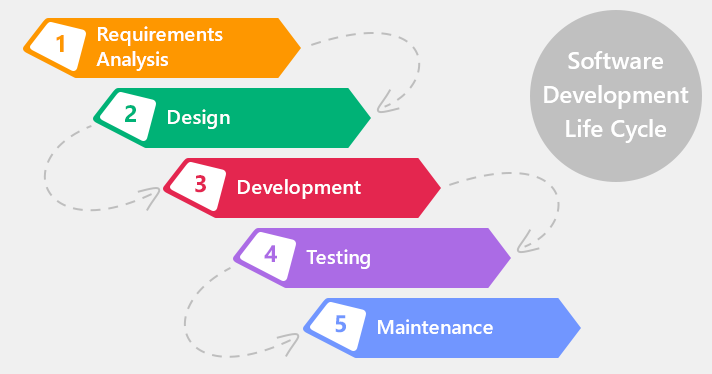
\includegraphics[width = 60mm]{lc.JPG}
\caption{This is a Life Cycle Model}
\label{Life Cucle Models}
\end{figure}

There are various life cycle models to improve the software processes. And we have used the WATERFALL MODEL.\\
This model contains\textbf{\textit{  6 phases:}}\\
o \textbf{\textit{ Feasibility study}}
The feasibility study activity involves the analysis of the problem and
collection of the relevant information relating to the product. The main aim
of the feasibility study is to determine whether it would be financially and
technically feasible to develop the product.\\
o \textbf{\textit{Requirement analysis }} and specification
The goal of this phase is to understand the exact requirements of the
customer and to document them properly.\\
o\textbf{\textit{ Design }}
The goal of this phase is to transform the requirement specification into a
structure that is suitable for implementation in some programming language.\\
o \textbf{\textit{Implementation }} and unit testing\\
During this phase the design is implemented. Initially small modules are
tested in isolation from rest of the software product.\\
o \textbf{\textit{ Integration and system testing}}\\
In this all the modules are integrated and then tested altogether.\\
o \textbf{\textit{Operation and maintenance. }} 
Release of software inaugurates the operation and life cycle phase of the
operation.\\
\subsubsection{ Agile development, Scrum.} 
Scrum was in the center of developing process.
As scrum projects make progress in a series of “sprints”, we have divided the whole process into
4 sprints. Product was first analysed, designed , then code and tested during the sprint. \\
Scrum
Roles \\
	•	Scrum Master – Prof.Dr. Olivier Biberstein\\
	•	Developer – Kristina Shiryagina\\
 Artifacts \\
	•	Product Backlog\\
	•	Sprint Backlog\\
 Meetings have included :\\
	•	Product/release planning\\
	•	Sprint planning\\
	•	Weekly Scrum\\
	•	Sprint review\\
	•	Sprint retrospective\\
Scrum Meetings \\
Each meeting between developer and scrum master was made of several steps, that were repeated each time:\\
	•	Attendance: all\\
	•	Product Owner presents Product Backlog\\
with all relevant user stories with their priority\\
	•	Discussions and clarifications if needed\\
	•	Results:\\
Prioritized Product Backlog\\
	•	Specifies what to build\\
	•	Final decision by the Master\\
	•	Vision, high level architecture, most important non-functional\\
requirements\\
Release planning (if product is to be delivered in releases):\\
	•	Select and prioritize items of Product Backlog for the next Release Backlog\\





 	 

\section{Conclusion and future work}
/**

*/
\lipsum[6-7]

%% print the bibliography and add the section to the table of content
\printbibliography[heading=bibintoc]

%%How I learned my ABCs\citep{ABCDE}.

\begin{thebibliography}{books}
\bibitem{ABCDE}Walter Abish \emph{The Alphabetical Africa},1974
\end{thebibliography}

\end{document}
